
\documentclass[tikz, convert={outfile=\jobname.png}]{standalone}

%% In /etc/ImageMagick-6/policy.xml
% change line:
% policy domain="coder" rights="none" pattern="PDF" 
% to:
% policy domain="coder" rights="read|write" pattern="PDF"

\begin{document}

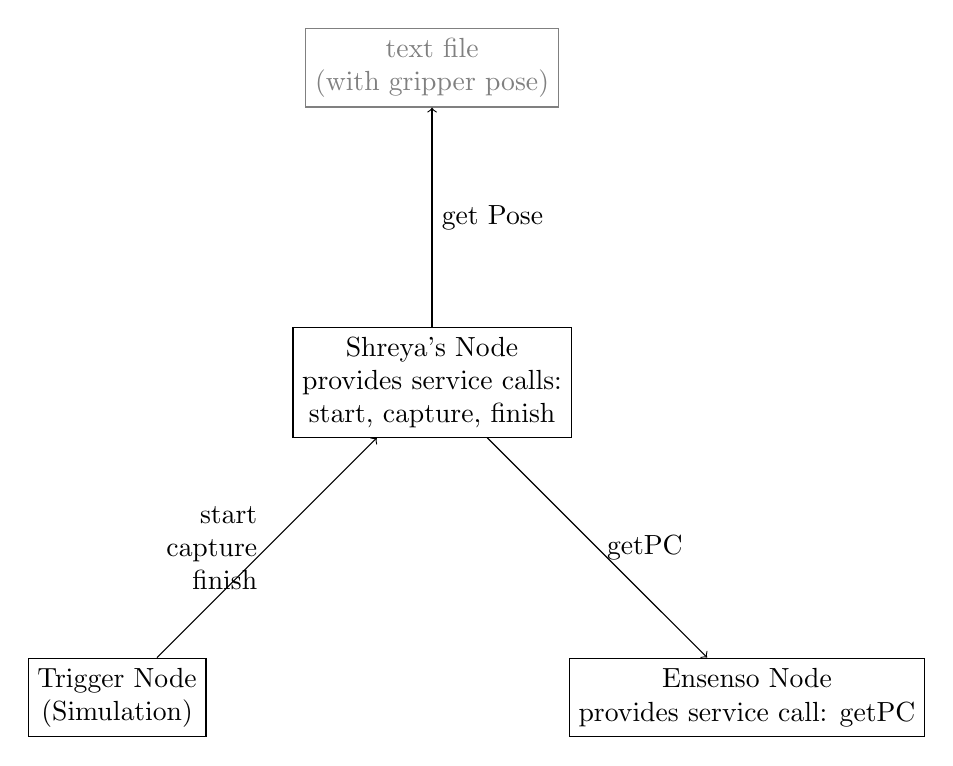
\begin{tikzpicture}[
block/.style={draw, align=center, minimum height=1cm, minimum width=2cm},
scale=2
]



\path (0,0) node[block](shreya){Shreya's Node \\ provides service calls: \\ start, capture, finish};
\path (2,-2) node[block](ensenso){Ensenso Node \\ provides service call: getPC};
\path (-2,-2) node[block](mikado){Trigger Node \\ (Simulation)};

\path (0,2) node[block, gray](text){text file \\ (with gripper pose)};



\draw[->] (mikado)--(shreya) node[midway, left, align=right] {start \\ capture \\ finish};
\draw[->] (shreya)--(ensenso) node[midway, right, align=left] {getPC};
\draw[->] (shreya)--(text) node[midway, right, align=left] {get Pose};






\end{tikzpicture}


\end{document}